% !TEX root = ../memorianueva.tex
% Chapter 4

\chapter{Ensayos y resultados} % Main chapter title

\label{Chapter4} % Para referenciar este capítulo: \ref{Chapter4}

En el presente capítulo se describen las pruebas realizadas sobre el sistema y los resultados obtenidos. Se presenta primero el plan de ensayos, con su metodología, sus instrumentos de medición y sus criterios de evaluación. Luego se exponen los ensayos de conectividad y comunicación, los de la capa de aplicación y los de integración extremo a extremo. El capítulo cierra con el análisis de los resultados, las limitaciones detectadas y las mejoras que se desprenden de ellas.

%----------------------------------------------------------------------------------------
%	SECTION 1
%----------------------------------------------------------------------------------------

\section{Plan de ensayos}
\label{sec:plan_ensayos}

El plan de ensayos se organizó en dos niveles complementarios. El primero corresponde a la verificación y reúne las pruebas orientadas a comprobar que cada componente fue construido de acuerdo con lo especificado. El segundo corresponde a la validación y reúne las pruebas ejecutadas sobre el sistema en operación real en el comercio, orientadas a comprobar que la solución resuelve el problema planteado.

\subsection{Alcance y ventanas de medición}
\label{subsec:alcance_medicion}

La condición particular de este trabajo es que el sistema se desplegó en producción y operó de forma continua durante el período de evaluación. Esa circunstancia permitió sustituir buena parte de los ensayos de laboratorio por mediciones sobre la operación real, con un volumen de casos muy superior al que habría aportado un banco de pruebas construido para la ocasión.

El sistema entró en operación el 1 de junio de 2026 y el primer pedido quedó registrado el 4 de junio. Sobre la ventana comprendida entre esa fecha y el 17 de agosto de 2026 se procesaron 3871 pedidos de 202 clientes, con un total de 29\,457 ítems y un promedio de 7,61 ítems por pedido.

Las mediciones no cubren todas un mismo intervalo, ya que cada subsistema conserva su información durante un lapso distinto.

En la tabla \ref{tab:ventanas} se detallan las tres ventanas empleadas y el motivo de su extensión.

\begin{table}[H]
    \centering
    \caption{Ventanas de medición empleadas en los ensayos.}
    \label{tab:ventanas}
    \begin{tabular}{L{4.9cm} L{3.1cm} c L{3.0cm}}
        \toprule
        \textbf{Aspecto medido}             & \textbf{Período}    & \textbf{Días} & \textbf{Limitación}                     \\
        \midrule
        Captura e interpretación de pedidos & 04/06 al 17/08/2026 & 75            & Inicio de la operación                  \\
        Impresión automática en el borde    & 29/06 al 17/08/2026 & 50            & Habilitación de la impresión automática \\
        Ejecuciones de la orquestación      & 04/08 al 17/08/2026 & 14            & Purga automática de ejecuciones         \\
        \bottomrule
    \end{tabular}
\end{table}

La diferencia entre la primera y la segunda ventana obedece a la puesta en marcha escalonada. Durante las cuatro primeras semanas la capa de captura e interpretación operó con el volumen completo de pedidos sin impresora térmica en el comercio, y los resultados se volcaron a un archivo de texto en la nube que el personal consultaba de forma manual. La actuación automática en el borde se habilitó en la semana del 29 de junio, una vez instalada la impresora y verificada la calidad de la interpretación, tras lo cual el volumen se estabilizó por encima de las quinientas operaciones semanales. Diferir la automatización hasta contar con esa evidencia constituyó una medida deliberada de reducción de riesgo operativo.

La tercera ventana responde a una restricción del registro de ejecuciones de la plataforma de orquestación, que conserva las ejecuciones durante 14 días y luego las elimina de forma automática. Sobre ese lapso se registraron 7036 ejecuciones y 789 pedidos.

\subsection{Instrumentos de medición}
\label{subsec:instrumentos}

La medición se apoyó en tres fuentes de información distintas.

La primera es la base de datos relacional del sistema, que registra cada pedido, cada ítem y cada intento de impresión con su marca temporal y su resultado: la tabla \code{print\_logs} conserva el estado de cada operación de impresión, y la ausencia de valor en el campo \code{producto\_id} de \code{items\_pedido} identifica los ítems no vinculados al catálogo. Esta fuente aporta la totalidad de la información de las secciones \ref{sec:ensayos_conectividad} y \ref{sec:ensayos_aplicacion}, aunque conserva el pedido ya estructurado y no el mensaje original.

La segunda es el registro de ejecuciones de la plataforma de orquestación, que conserva el instante de inicio y de finalización de cada flujo junto con su estado final. Esa información permite acotar el tiempo de interpretación, que no queda registrado en la base relacional del sistema.

La tercera es la plataforma de atención vinculada al canal de mensajería, que conserva cada mensaje entrante con su marca temporal, su contacto de origen y el tipo de contenido de sus adjuntos. Esa fuente aporta la única información disponible sobre el formato del mensaje original, dimensión que las dos anteriores no permiten discriminar, y sostiene la auditoría de la subsección \ref{subsec:ensayo_formatos}. Su vinculación con los pedidos no es directa, ya que ambos sistemas no comparten identificadores, y debió reconstruirse por coincidencia del número de contacto y proximidad temporal según el procedimiento que allí se detalla.

\subsection{Estrategia de verificación adoptada}
\label{subsec:estrategia_verificacion}

Los requerimientos de testing previeron la ejecución de pruebas unitarias sobre los módulos de procesamiento e impresión y de pruebas de integración entre los componentes. La revisión del repositorio confirmó que no se implementaron conjuntos de pruebas automatizadas, más allá del archivo de ejemplo que genera el entorno de desarrollo del panel, que no contiene casos de prueba.

En su reemplazo, la verificación se apoyó en la operación real del sistema durante 75 días. Esa estrategia aporta una cobertura de casos superior a la que habría alcanzado un conjunto de pruebas construido para la ocasión, con la variabilidad propia de los mensajes de clientes reales, y permite validar de forma simultánea la integración de todos los componentes. Su limitación es que no detecta regresiones de manera anticipada ni permite aislar la causa de una falla en un componente determinado, motivo por el que la incorporación de pruebas automatizadas se propone como trabajo futuro en el capítulo \ref{Chapter5}.

\subsection{Criterios de evaluación}
\label{subsec:criterios}

La planificación del trabajo definió, para cada requerimiento, un método de verificación y un método de validación, pero no estableció valores numéricos de corte con anterioridad al desarrollo. Los ensayos descriptos en este capítulo son, en consecuencia, de caracterización: se orientan a determinar el comportamiento efectivo del sistema en operación antes que a contrastarlo contra umbrales preestablecidos.

El criterio de aceptación que operó de manera efectiva fue la validación por parte del cliente en el entorno real. El sistema se incorporó a la operación diaria del comercio y permaneció en uso continuo durante todo el período analizado, lo que constituye una forma de aceptación por uso sostenido. En la subsección \ref{subsec:verificacion_requerimientos} se contrasta cada requerimiento contra la evidencia obtenida.

%----------------------------------------------------------------------------------------
%	SECTION 2
%----------------------------------------------------------------------------------------

\section{Ensayos de conectividad y comunicación}
\label{sec:ensayos_conectividad}

Los ensayos de conectividad se orientaron a verificar el vínculo entre la nube y el nodo de borde, que constituye el único punto de contacto entre ambos entornos y, por lo tanto, el eslabón crítico de la cadena. La medición se apoyó en la operación real: cada intento de envío de un ticket hacia el servidor local quedó registrado con su resultado y, en caso de falla, con el mensaje de error devuelto.

\subsection{Confiabilidad del vínculo en operación}
\label{subsec:confiabilidad_vinculo}

El análisis distingue el período de prueba de la impresora del período de operación automática, ya que las condiciones difieren por completo. Durante las cuatro primeras semanas, cuando el comercio aún no contaba con el equipo, se registraron 39 operaciones de impresión, de las que 13 finalizaron con error. Esos casos carecen de valor para evaluar la confiabilidad del vínculo, dado que el destino de la orden no existía.

Durante el período de operación automática, comprendido entre el 29 de junio y el 17 de agosto, se registraron 4334 operaciones de impresión, de las que 22 finalizaron con error, lo que arroja una tasa de fallas del 0,51 por ciento.
En la tabla \ref{tab:errores_conectividad} se detalla la clasificación de los errores del período de operación automática según su mensaje y su origen.

\begin{table}[H]
    \centering
    \caption{Clasificación de los errores registrados durante la operación automática.}
    \label{tab:errores_conectividad}
    \begin{tabular}{l L{6.2cm} c}
        \toprule
        \textbf{Mensaje}  & \textbf{Origen}               & \textbf{Casos} \\
        \midrule
        HTTP 530          & Túnel sin origen alcanzable   & 18             \\
        HTTP 502          & Pasarela intermedia           & 2              \\
        HTTP 520          & Respuesta inválida del origen & 1              \\
        Fallo de conexión & Red entre la nube y el túnel  & 1              \\
        \midrule
        Total             &                               & 22             \\
        \bottomrule
    \end{tabular}
\end{table}

La totalidad de los errores del período de operación automática corresponde a interrupciones del vínculo de comunicación. Los códigos 530 y 520 son emitidos por el proveedor del túnel cuando el extremo local no responde, situación que se produce ante una caída de la conexión a Internet del comercio o ante la detención del proceso en el servidor local. Ningún error se originó en la impresora ni en el formateo del ticket, lo que indica que la actuación física en el borde resultó estable durante todo el período.

Este comportamiento respalda el criterio de distribución del cómputo adoptado en la subsección \ref{subsec:criterio_distribucion}. La única dependencia externa del proceso de impresión es la llegada de la orden desde la nube, y una vez que esa orden alcanza el nodo de borde la operación se completa sin intermediarios.

\subsection{Análisis de los episodios de pérdida de conectividad}
\label{subsec:episodios_conectividad}

La distribución temporal de los errores resultó más informativa que su recuento. Los 22 casos no se presentaron de forma aislada sino agrupados en episodios de indisponibilidad del vínculo, según se detalla en la tabla \ref{tab:episodios}.

\begin{table}[H]
    \centering
    \caption{Episodios de pérdida de conectividad registrados durante la operación automática.}
    \label{tab:episodios}
    \begin{tabular}{l c c c c}
        \toprule
        \textbf{Fecha} & \textbf{Duración} & \textbf{Pedidos afectados} & \textbf{Mensaje}  & \textbf{Sin ticket} \\
        \midrule
        11/07/2026     & 1\,h 12\,min      & 9                          & HTTP 530          & 8                   \\
        13/07/2026     & Aislado           & 1                          & HTTP 502          & 0                   \\
        18/07/2026     & Aislado           & 1                          & HTTP 520          & 1                   \\
        24/07/2026     & Aislado           & 1                          & Fallo de conexión & 0                   \\
        27/07/2026     & Aislado           & 1                          & HTTP 530          & 0                   \\
        28/07/2026     & 1\,h 25\,min      & 5                          & HTTP 530          & 5                   \\
        29/07/2026     & 8\,min            & 3                          & HTTP 502 y 530    & 1                   \\
        \midrule
        Total          &                   & 21                         &                   & 15                  \\
        \bottomrule
    \end{tabular}
\end{table}

Los dos episodios prolongados concentran 14 de los 21 pedidos afectados y presentan un patrón coherente con una interrupción del servicio de Internet en el comercio: fallas consecutivas sobre pedidos distintos, mismo código de error y cese simultáneo al finalizar el episodio. Los casos aislados se resolvieron en plazos que van de los 12 segundos a las 16 horas.

El registro de impresiones marca los 22 casos como atendidos, pero esa marca refleja la resolución operativa del personal, no la emisión del ticket: tres de los pedidos afectados ya tenían un ticket emitido (la falla fue sobre una reimpresión), otros tres lo recibieron después del episodio, y los 15 restantes, el 0,39 por ciento de los 3871 pedidos del período, no registran ninguna emisión exitosa y se armaron sin comprobante impreso.

La indisponibilidad del vínculo no interrumpe la operación, ya que el pedido permanece accesible en el panel y el personal puede continuar el armado, pero el sistema carece de un mecanismo de reintento automático y la recuperación depende de que el personal advierta la falta del ticket. Como el enlace se restablece por sí solo en plazos acotados, una cola de reintentos, la mejora propuesta en la subsección \ref{subsec:mejoras_ensayos}, resolvería el problema sin intervención.

%----------------------------------------------------------------------------------------
%	SECTION 3
%----------------------------------------------------------------------------------------

\section{Ensayos de la capa de aplicación}
\label{sec:ensayos_aplicacion}

Los ensayos de la capa de aplicación se orientaron a evaluar dos dimensiones. La primera es la calidad de la interpretación de los pedidos, que constituye la función central del sistema. La segunda es la estabilidad de la plataforma de orquestación que coordina esa interpretación.

\subsection{Tasa de reconocimiento de ítems}
\label{subsec:tasa_reconocimiento}

La métrica adoptada para evaluar la interpretación fue la proporción de ítems que el agente logró asociar con un producto del catálogo del comercio. Un ítem no asociado se registra con la denominación original recibida y se destaca en el panel, de modo que la operación continúa pero requiere una decisión del personal.

Sobre un total de 29\,457 ítems procesados durante los 75 días de operación, 28\,999 fueron asociados con un producto del catálogo, lo que arroja una tasa de reconocimiento del 98,45 por ciento. Los 458 ítems restantes quedaron sin asociar y se distribuyeron en 213 denominaciones distintas.

\subsection{Análisis de los ítems no reconocidos}
\label{subsec:items_no_reconocidos}

Las denominaciones no asociadas se clasificaron mediante su normalización, con supresión de tildes y unificación de mayúsculas, y su posterior comparación contra el catálogo de productos. El análisis permite distinguir ocho situaciones de naturaleza distinta, que se detallan en la tabla \ref{tab:no_reconocidos}.

La primera situación reúne nombres de variedad y códigos de calibre propios del comercio mayorista de frutas, como las variedades de mandarina Ellendale y Encore (38 casos) y de pera Bosc (18 casos), ninguna con correspondencia en el catálogo. Las escrituras registradas son además inconsistentes, con Ellendale bajo nueve variantes y Bosc bajo 15, un patrón compatible con la transcripción de listas con terminología ausente del catálogo.

\begin{table}[H]
    \centering
    \caption{Clasificación de los ítems no asociados al catálogo.}
    \label{tab:no_reconocidos}
    \begin{tabular}{L{8.2cm} c c}
        \toprule
        \textbf{Situación}                                 & \textbf{Casos} & \textbf{Porcentaje} \\
        \midrule
        Variedades comerciales y códigos de calibre        & 112            & 0,38                \\
        Producto incorporado al catálogo con posterioridad & 94             & 0,32                \\
        Productos de almacén ausentes del catálogo         & 82             & 0,28                \\
        Denominaciones sin correspondencia interpretable   & 80             & 0,27                \\
        Frutas y hortalizas ausentes del catálogo          & 47             & 0,16                \\
        Producto presente en el catálogo pero inactivo     & 29             & 0,10                \\
        Contenido ilegible en el mensaje de origen         & 9              & 0,03                \\
        Casos residuales posteriores al alta del producto  & 5              & 0,02                \\
        \midrule
        Total                                              & 458            & 1,55                \\
        \bottomrule
    \end{tabular}
\end{table}

La segunda situación agrupa 94 ítems de productos que no integraban el catálogo al momento del pedido y se incorporaron después. El caso del huevo es ilustrativo: 55 ocurrencias no asociadas entre el 10 de junio y el 12 de julio, sin fallos posteriores a su alta. El patrón evidencia un mecanismo de realimentación operativa, en el que los ítems que el panel destaca orientan la ampliación progresiva del catálogo.

La tercera, la quinta y la sexta situación corresponden a productos ausentes del catálogo o dados de baja: de almacén (cúrcuma, 15 casos, y otros condimentos), frescos (hongo portobello, 17 casos) e inactivos (miel y pimentón, entre los más frecuentes de 29 casos). En los tres casos la interpretación del agente fue adecuada y la falta de asociación refleja una limitación de cobertura, no un error de lectura.

La séptima situación corresponde a los mensajes cuyo contenido no pudo leerse (9 casos), resultado del diseño del agente, instruido para señalar la imposibilidad de lectura en lugar de inferir un producto probable, ya que un ítem incorrecto genera un error de armado mientras que uno señalado como dudoso deriva en una consulta previa al cliente. Los 5 casos residuales se registraron en los días posteriores al alta de un producto.

La conclusión modifica de forma sustancial la lectura del 1,55 por ciento de ítems no asociados: 364 de los 458 responden a la cobertura del catálogo y 9 a contenido ilegible señalado de forma deliberada. Únicamente los 80 casos sin correspondencia interpretable son atribuibles a un error de interpretación, el 0,27 por ciento de los ítems procesados, lo que sitúa la exactitud efectiva de la interpretación en el 99,73 por ciento.

\subsection{Estabilidad de la orquestación}
\label{subsec:estabilidad_orquestacion}

La plataforma de orquestación coordina la recepción de los mensajes, la invocación de los modelos de interpretación y la persistencia de los pedidos. Su registro de ejecuciones permite evaluar la estabilidad del conjunto. En la tabla \ref{tab:flujos} se resumen las ejecuciones registradas durante la ventana de 14 días.

\begin{table}[H]
    \centering
    \caption{Ejecuciones registradas por flujo de orquestación.}
    \label{tab:flujos}
    \begin{tabular}{L{5.6cm} c c c}
        \toprule
        \textbf{Flujo}              & \textbf{Correctas} & \textbf{Con error} & \textbf{Duración media} \\
        \midrule
        Interpretación de pedidos   & 6710               & 2                  & 36,31\,s                \\
        Confirmación de pedidos     & 299                & 4                  & 0,87\,s                 \\
        Sincronización de contactos & 13                 & 1                  & 3627,05\,s              \\
        Gestión de errores          & 7                  & 0                  & 0,49\,s                 \\
        \midrule
        Total                       & 7029               & 7                  &                         \\
        \bottomrule
    \end{tabular}
\end{table}

Sobre 7036 ejecuciones se registraron 7 fallas, lo que arroja una tasa de error del 0,10 por ciento. Ese valor verifica el requerimiento de integración entre los componentes, ya que cada ejecución del flujo de interpretación involucra al canal de mensajería, a la base en memoria, a los servicios de inteligencia artificial y a la base relacional.

La duración media del flujo de interpretación no debe leerse como tiempo de procesamiento, según se analiza en la subsección \ref{subsec:composicion_latencia}.

El flujo de sincronización de contactos, que actualiza de forma programada los nombres de los clientes a partir de la agenda del comercio, presenta una duración media del orden de la hora, con 13 ejecuciones en 14 días. Ese valor no refleja un costo de cómputo sino las esperas deliberadas que el flujo intercala entre lotes para respetar los límites de tasa de las interfaces que consume. Al operar de forma desacoplada del flujo de pedidos, no incide sobre la latencia percibida por el comercio.

%----------------------------------------------------------------------------------------
%	SECTION 4
%----------------------------------------------------------------------------------------

\section{Ensayos de integración extremo a extremo}
\label{sec:ensayos_integracion}

Los ensayos de integración evalúan el recorrido completo del pedido, desde la recepción del mensaje hasta la emisión del ticket en el comercio. El análisis se organiza en dos partes. La primera mide la latencia de la actuación en el borde, que es la etapa que el diseño buscó optimizar. La segunda descompone la latencia total y acota la contribución de cada tramo.

\subsection{Latencia de la actuación en el borde}
\label{subsec:latencia_borde}

Se midió el tiempo transcurrido entre la persistencia del pedido en la base de datos y la emisión de su primer ticket. En la figura \ref{fig:latencia_impresion} se presenta la distribución obtenida sobre 2606 pedidos.

La distribución resultó marcadamente bimodal. El 98,58 por ciento de los casos se resolvió en menos de cinco segundos y el 1,38 por ciento superó el minuto, mientras que en el intervalo intermedio, que abarca casi un minuto completo, se registró un único caso. Esa discontinuidad indica la presencia de dos poblaciones de naturaleza distinta y permite separarlas mediante un umbral de cinco segundos, cuya ubicación dentro de un intervalo vacío vuelve irrelevante la elección precisa del valor.

\begin{figure}[H]
    \centering
    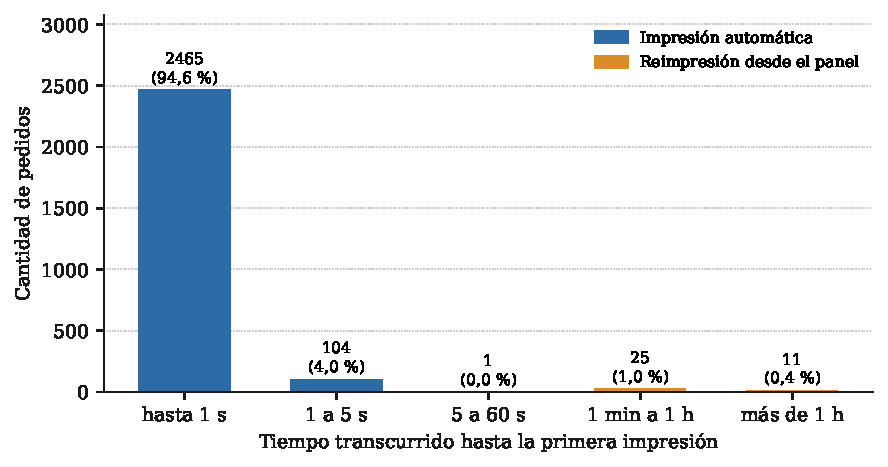
\includegraphics[width=0.9\textwidth]{Figures/latencia_impresion.pdf}
    \caption{Distribución del tiempo transcurrido entre la persistencia del pedido y su primera impresión.}
    \label{fig:latencia_impresion}
\end{figure}

La primera población corresponde a la impresión automática que el sistema dispara al persistir el pedido. La segunda corresponde a la reimpresión diferida que el personal ejecuta desde el panel, en general con precios incluidos, en el momento del despacho. Esa interpretación se confirma al observar que 1321 pedidos registraron exactamente dos impresiones, cantidad superior a los 1113 pedidos con una sola, y que 1621 de las impresiones correctas se emitieron con precios frente a 2717 sin ellos. La doble emisión responde al flujo operativo del comercio, que utiliza un ticket sin precios para el armado del pedido y otro con precios para su entrega.

En la tabla \ref{tab:latencias} se presentan las métricas correspondientes a la población de impresión automática.

\begin{table}[H]
    \centering
    \caption{Latencia de la impresión automática en el borde.}
    \label{tab:latencias}
    \begin{tabular}{L{5.5cm} c}
        \toprule
        \textbf{Métrica} & \textbf{Valor} \\
        \midrule
        Casos analizados & 2569           \\
        Mínimo           & 0,110\,s       \\
        Media            & 0,425\,s       \\
        Mediana          & 0,338\,s       \\
        Percentil 95     & 0,921\,s       \\
        Percentil 99     & 1,475\,s       \\
        Máximo           & 4,220\,s       \\
        \bottomrule
    \end{tabular}
\end{table}

El resultado más significativo no es la mediana sino la dispersión. El peor caso registrado en 50 días de operación fue de 4,22 segundos, y la coincidencia entre media y mediana indica una distribución sin cola apreciable. La actuación física del sistema resultó, por lo tanto, no solo rápida sino predecible.

Ese comportamiento es consecuencia directa del criterio de distribución del cómputo. La orden de impresión recorre un único salto dentro de la red del comercio y no atraviesa Internet, de modo que su latencia queda determinada por la red local y por el tiempo de respuesta de la impresora.

\subsection{Composición de la latencia extremo a extremo}
\label{subsec:composicion_latencia}

La latencia total percibida por el comercio se compone de dos tramos. El primero abarca desde la recepción del mensaje hasta la persistencia del pedido y se resuelve en la nube. El segundo abarca desde la persistencia hasta la emisión del ticket y se resuelve en el borde, con los valores de la sección anterior.

El primer tramo se midió a partir de la duración de las ejecuciones del flujo de interpretación. En la figura \ref{fig:latencia_orquestacion} se presenta su distribución.

\begin{figure}[H]
    \centering
    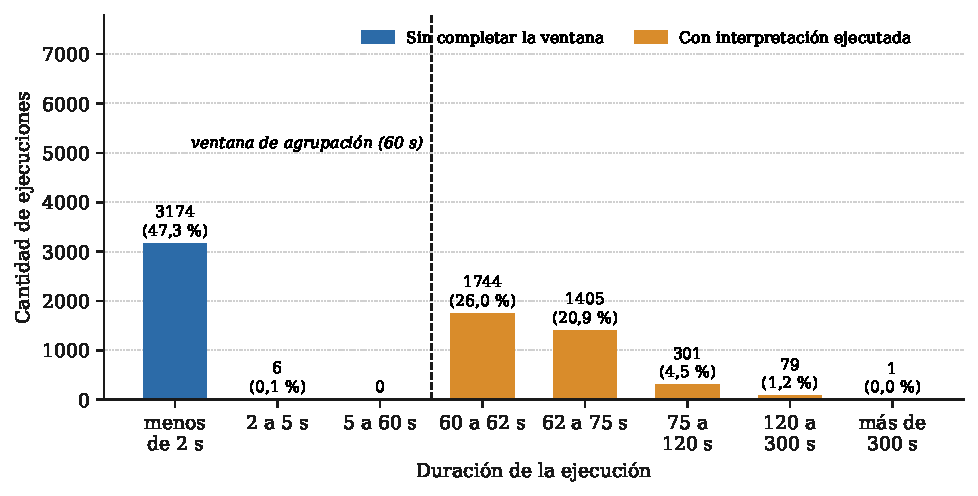
\includegraphics[width=0.9\textwidth]{Figures/latencia_orquestacion.pdf}
    \caption{Distribución de la duración de las ejecuciones del flujo de interpretación de pedidos.}
    \label{fig:latencia_orquestacion}
\end{figure}

La distribución vuelve a presentar dos poblaciones separadas por un intervalo vacío. El 47,39 por ciento de las ejecuciones finalizó en menos de cinco segundos y el 52,61 por ciento restante superó los 60, sin ningún caso registrado entre ambos valores.

La explicación se encuentra en el mecanismo de agrupación de mensajes descripto en la subsección \ref{subsec:criterio_distribucion}. Ese mecanismo no impone una espera fija sino una espera por inactividad. Cada mensaje entrante se incorpora a una lista asociada al cliente y la ejecución aguarda 60 segundos antes de reevaluar el estado de esa lista. Si durante ese lapso llegó un mensaje posterior, la ejecución concluye sin procesar y delega la interpretación en la ejecución más reciente. Si no llegó ninguno, procede a interpretar el conjunto completo y elimina la lista.

La distribución permite entonces distinguir tres comportamientos. Las 3180 ejecuciones que finalizaron en menos de cinco segundos corresponden a mensajes descartados por los filtros previos, que excluyen los mensajes de grupos y los emitidos por el propio comercio. Las 1744 comprendidas entre 60 y 62 segundos corresponden a mensajes sucesivos de un mismo pedido, que concluyeron al detectar la llegada de un mensaje posterior. Las 1786 restantes son las que ejecutaron efectivamente la interpretación, y de ellas 1405 completaron el procesamiento en menos de 15 segundos adicionales a la espera, 301 lo hicieron entre 15 y 60, 79 entre 60 y 240, y una sola superó ese valor.

El tiempo de cómputo de la interpretación se ubica, por lo tanto, en el orden de las unidades de segundo. La demora dominante en el tramo que se resuelve en la nube no proviene del procesamiento sino de la espera deliberada por inactividad del cliente.

El contraste entre ambos tramos constituye el resultado central del trabajo. La etapa que depende de servicios remotos admite una espera de 60 segundos porque su restricción no es de latencia sino de completitud del pedido, mientras que la etapa que ejecuta la actuación física en el borde opera con un máximo de 4,22 segundos y una mediana inferior al medio segundo. La distribución del cómputo asignó a cada entorno la tarea que mejor se ajusta a sus características.

Corresponde precisar qué unidad mide esta distribución, ya que 1786 ejecuciones completaron la interpretación frente a 789 pedidos persistidos, una relación de 2,26 ejecuciones por pedido. La reconstrucción de las agrupaciones que el mecanismo de espera habría formado sobre los 3386 mensajes de la ventana arroja 1801 con un corte de 90 segundos, valor que difiere en menos del uno por ciento de esas 1786 ejecuciones.

La coincidencia establece que cada ejecución de interpretación corresponde a una conversación agrupada y no a un pedido. Las 997 conversaciones restantes son intercambios que superaron los filtros previos pero no derivaron en un encargo, como consultas de precio, confirmaciones y saludos. La duración medida es, en consecuencia, la del procesamiento de una conversación, y el sistema resuelve algo más del doble de conversaciones que de pedidos.

\subsection{Auditoría por formato de entrada}
\label{subsec:ensayo_formatos}

El requerimiento de admitir pedidos en texto, voz, imagen y documento exige comparar el comportamiento del sistema entre esas cuatro modalidades. Ninguna de las dos primeras fuentes de medición lo permite, ya que la base relacional conserva el pedido ya estructurado y no el mensaje que lo originó. La comparación se construyó, en consecuencia, sobre el registro de la plataforma de atención, que sí conserva el tipo de contenido de cada mensaje entrante.

\subsubsection*{Reconstrucción del vínculo entre mensaje y pedido}

Los dos sistemas no comparten identificadores, por lo que la correspondencia entre un mensaje y el pedido se reconstruyó emparejando cada pedido con el último mensaje entrante del mismo contacto anterior a su registro, aprovechando el mecanismo de agrupación por inactividad de la subsección \ref{subsec:composicion_latencia}. La distancia mediana entre ambos es de 72 segundos (primer cuartil 68, tercer cuartil 85), coherente con la espera de 60 segundos más el procesamiento. Se consideraron atribuibles los pedidos con un mensaje precedente a no más de 120 segundos, criterio que alcanza a 3038 de los 3871 pedidos de la ventana (78,48 por ciento).

La cobertura del emparejamiento se mantuvo estable a lo largo del período (mediana diaria del 79 por ciento, mínimo del 61 por ciento), sin días anómalos, lo que descarta que el subconjunto atribuido corresponda a un tramo particular de la operación.

\subsubsection*{Composición del tráfico y resultados por formato}

Durante la ventana de 75 días se recibieron 16\,619 mensajes entrantes de contactos individuales. De ese total, el 77,39 por ciento fue texto, el 12,41 por ciento audio, el 8,29 por ciento imagen, el 1,78 por ciento documento y el 0,14 por ciento video. Las cuatro modalidades previstas por el requerimiento se presentan, por lo tanto, en la operación real y con volumen suficiente para ser comparadas, con la salvedad del video, cuya presencia es marginal.

En la tabla \ref{tab:formatos} se presentan los resultados de la auditoría sobre los 3038 pedidos atribuidos. La categoría mixta reúne los pedidos cuya agrupación combina adjuntos de más de un tipo.

\begin{table}[H]
    \centering
    \caption{Auditoría por formato de entrada sobre los pedidos atribuidos.}
    \label{tab:formatos}
    \begin{tabular}{l c c c c c}
        \toprule
        \textbf{Formato} & \textbf{Pedidos} & \textbf{\%} & \textbf{Ítems} & \textbf{Tasa de asociación} & \textbf{Ítems/pedido} \\
        \midrule
        Texto            & 2013             & 66,26       & 12\,060        & 99,17                       & 5,99                  \\
        Audio            & 563              & 18,53       & 2952           & 99,32                       & 5,24                  \\
        Imagen           & 405              & 13,33       & 4727           & 99,30                       & 11,67                 \\
        Mixto            & 40               & 1,32        & 321            & 98,75                       & 8,03                  \\
        Documento        & 16               & 0,53        & 424            & 98,11                       & 26,50                 \\
        Video            & 1                & 0,03        & 1              & 100,00                      & 1,00                  \\
        \midrule
        Total            & 3038             & 100,00      & 20\,485        & 99,19                       & 6,74                  \\
        \bottomrule
    \end{tabular}
\end{table}

El resultado principal es la ausencia de diferencias apreciables en la tasa de asociación entre las tres modalidades de volumen significativo. El texto alcanza el 99,17 por ciento, el audio el 99,32 y la imagen el 99,30, valores comprendidos en un intervalo de 0,15 puntos porcentuales. El documento presenta el valor más bajo, 98,11 por ciento, pero sobre una base de 16 pedidos que no admite generalización. La interpretación multimodal no introduce, en consecuencia, una penalización medible respecto del texto plano, que constituye el resultado de mayor relevancia para el requerimiento.

El segundo resultado es que el formato sí determina el tamaño del pedido. Un pedido enviado por texto contiene en promedio 5,99 ítems y uno enviado por audio 5,24, mientras que uno enviado por imagen contiene 11,67 y uno enviado como documento 26,50. Las modalidades de imagen y documento concentran los pedidos extensos, que son los que el comercio recibe como lista completa de reposición, y su aporte al volumen total de ítems resulta muy superior al que sugiere su participación en la cantidad de pedidos: la imagen representa el 13,33 por ciento de los pedidos pero el 23,08 por ciento de los ítems.

La combinación de ambos resultados corrige la lectura planteada como hipótesis en la subsección \ref{subsec:items_no_reconocidos}. El error residual no se concentra en la modalidad de imagen. Lo que la imagen concentra son los pedidos extensos con terminología de proveedor, de modo que la asociación entre listas manuscritas y denominaciones no interpretables responde al contenido de esos pedidos y no a una degradación de la interpretación por el hecho de provenir de una fotografía.

\subsubsection*{Limitaciones de la auditoría}

Tres limitaciones acotan el alcance de estos resultados y deben declararse de forma explícita.

La primera es que el indicador es la tasa de asociación con el catálogo, no la exactitud de la interpretación: un ítem asociado puede tener una cantidad o unidad incorrecta que ninguna fuente registra, y verificarlo exigiría contrastar cada pedido contra el mensaje original, viable solo por muestreo manual sobre este volumen.

La segunda es que el tiempo extremo a extremo no puede desagregarse por formato, ya que el registro de ejecuciones no discrimina la modalidad procesada, lo que impide aislar el costo de la transcripción de audio o de la lectura de imagen dentro de la latencia total.

La tercera es que el 21,52 por ciento de los pedidos de la ventana no pudo atribuirse a ningún mensaje próximo. Ese conjunto tiene pedidos más grandes (10,78 ítems) y menor asociación (96,75 por ciento), por lo que su exclusión eleva el valor global de la muestra auditada por encima del 98,45 por ciento real. La comparación entre formatos no se ve afectada porque el sesgo opera por igual sobre todos, pero los valores de la tabla \ref{tab:formatos} no deben leerse como la tasa de asociación del sistema, reportada en la subsección \ref{subsec:items_no_reconocidos}.

\subsection{Ensayo de interfaz}
\label{subsec:ensayo_interfaz}

El acceso al panel sin instalación adicional y su adaptación a distintos tamaños de pantalla se verificaron con un recorrido funcional en Google Chrome, Mozilla Firefox y Microsoft Edge, y en dos anchos de pantalla representativos de un teléfono (375\,px) y una tablet (768\,px).

El recorrido de las vistas de tablero, pedidos, detalle de pedido, productos, clientes y estadísticas no arrojó errores ni advertencias en la consola de ninguno de los tres navegadores. En el ancho de tablet el panel se comportó de forma equivalente al escritorio, dado el tamaño de pantalla similar; el menú lateral se colapsa en un menú desplegable y los controles resultan operables con el dedo. En el ancho de teléfono el panel es utilizable, sin errores ni elementos rotos, aunque algunas vistas con tablas extensas requieren desplazamiento horizontal, una oportunidad de mejora de la experiencia antes que una falla funcional.

El panel cumple, en consecuencia, con el acceso sin instalación adicional y con una adaptación funcional a los tres tamaños de pantalla evaluados. Las capturas del anexo \ref{AppendixA} documentan el estado de las vistas recorridas, de la figura \ref{fig:panel_tablero} a la \ref{fig:panel_metricas}, junto con el ticket emitido en el comercio (figura \ref{fig:ticket_real}).

\subsection{Trazabilidad del pedido}
\label{subsec:trazabilidad}

La trazabilidad se verificó de forma estructural. Cada pedido conserva el conjunto de ítems interpretados, con su denominación original cuando no pudieron asociarse al catálogo, el texto exacto enviado a la impresora y el registro completo de los intentos de impresión con su resultado, su marca temporal y su eventual mensaje de error. El panel permite además acceder desde cada pedido al hilo de la conversación que le dio origen.

La consecuencia práctica de ese diseño es que la totalidad de las mediciones presentadas en este capítulo pudo obtenerse a partir de la propia base de datos del sistema, sin instrumentación adicional. La trazabilidad no solo satisface el requerimiento correspondiente, sino que constituyó el instrumento de medición principal del trabajo.

La cadena presenta, sin embargo, una discontinuidad. El mensaje original recibido del cliente no se persiste en la base relacional, que almacena el pedido ya estructurado, sino que permanece únicamente en la plataforma de atención vinculada al canal de mensajería. La reconstrucción del recorrido completo exige, en consecuencia, consultar dos sistemas distintos.

%----------------------------------------------------------------------------------------
%	SECTION 5
%----------------------------------------------------------------------------------------

\section{Análisis de resultados}
\label{sec:analisis_resultados}

Los ensayos anteriores aportan la evidencia con la que se cierra el capítulo. Esta sección la ordena en tres planos: contrasta cada requerimiento con la medición que lo respalda, reúne las limitaciones que esa medición dejó a la vista y deriva de ellas las mejoras propuestas.

\subsection{Verificación de los requerimientos}
\label{subsec:verificacion_requerimientos}

Los requerimientos se agrupan según la naturaleza de la evidencia. La tabla \ref{tab:verificacion} reúne los que se contrastaron con una medición cuantitativa sobre la operación real.

\begin{table}[H]
    \centering
    \caption{Requerimientos verificados por medición.}
    \label{tab:verificacion}
    \begin{tabular}{c L{5.8cm} L{6.0cm}}
        \toprule
        \textbf{Req.} & \textbf{Evidencia}                                     & \textbf{Resultado}                                                                               \\
        \midrule
        1.2           & Auditoría por formato de entrada.                      & Cuatro formatos en operación; asociación de 99,17 a 99,32 por ciento sin diferencia entre ellos. \\
        1.3           & Tasa de asociación de ítems con el catálogo.           & 98,45 por ciento sobre 29\,457 ítems.                                                            \\
        1.6           & Operaciones de impresión y pedidos sin ticket emitido. & 99,49 por ciento de 4334 operaciones; 15 sin ticket (0,39 por ciento).                           \\
        1.7           & Episodios de pérdida del vínculo con el borde.         & Siete episodios en 50 días, 21 pedidos afectados.                                                \\
        1.11          & Registro de ítems, ticket e impresiones.               & Verificado con una discontinuidad.                                                               \\
        3.1           & Pruebas unitarias automatizadas.                       & No implementadas.                                                                                \\
        3.2           & Tasa de error de la orquestación.                      & 0,10 por ciento sobre 7036 ejecuciones.                                                          \\
        3.3           & Operación en el comercio durante 75 días.              & 3871 pedidos de 202 clientes.                                                                    \\
        3.4           & Impresiones sin fallas atribuibles a la impresora.     & Verificado.                                                                                      \\
        3.5           & Latencia de la actuación en el borde.                  & Mediana de 0,338\,s.                                                                             \\
        \bottomrule
    \end{tabular}
\end{table}

La tabla \ref{tab:verificacion_funcional} reúne los requerimientos verificados por comprobación funcional cuyo resultado aporta algo más que el cumplimiento. Los restantes se omiten por no arrojar un resultado distinto de este: la persistencia y el uso de Redis de las subsecciones \ref{subsec:modelo_datos} y \ref{subsec:agrupacion} (1.4 y 1.5), el panel con sus alertas y su configuración del catálogo de la subsección \ref{subsec:panel} (1.9, 1.10 y 4.2), el acceso sin instalación de la subsección \ref{subsec:ensayo_interfaz} (4.1) y el versionado de los flujos (5.3).

\begin{table}[H]
    \centering
    \caption{Requerimientos verificados de forma funcional.}
    \label{tab:verificacion_funcional}
    \begin{tabular}{c L{5.8cm} L{6.0cm}}
        \toprule
        \textbf{Req.} & \textbf{Evidencia}                                                   & \textbf{Resultado}                                               \\
        \midrule
        1.1           & Recepción y procesamiento continuo de pedidos por WhatsApp.          & Verificado; 3871 pedidos de 202 clientes en 75 días.             \\
        1.8           & Ticket con datos del cliente, productos, aclaraciones, fecha y hora. & Verificado; anexo \ref{AppendixA}, figura \ref{fig:ticket_real}. \\
        4.3           & Adaptación a distintos tamaños de pantalla.                          & Verificado; con \textit{scroll} horizontal en teléfono.          \\
        5.1           & Compatibilidad con la API oficial de WhatsApp Business.              & Diseño compatible; migración no ejecutada.                       \\
        5.2           & Soporte para múltiples dispositivos o cuentas.                       & No evaluado con la evidencia disponible.                         \\
        \bottomrule
    \end{tabular}
\end{table}

El balance es que todos los requerimientos verificables quedaron satisfechos, con una excepción y una salvedad: las pruebas unitarias automatizadas del requerimiento 3.1, cuya función cubrió la operación real sin capacidad de detectar regresiones, y el requerimiento 1.11, verificado con la discontinuidad que introduce la ausencia del mensaje original en la base relacional.

\FloatBarrier

\subsection{Limitaciones detectadas}
\label{subsec:limitaciones}

El conjunto de ensayos permitió identificar seis limitaciones.

La primera es la dependencia del estado del catálogo. La cobertura incompleta y la baja de productos vigentes explican 364 de los 458 ítems no asociados, el 79,48 por ciento: productos incorporados con posterioridad, de almacén y frescos ausentes, dados de baja y las variedades comerciales y códigos de calibre que se retoman en la limitación siguiente. El sistema carece de un mecanismo que anticipe esa condición, de modo que la incorporación ocurre siempre después del primer pedido que la solicita.

La segunda es la cobertura frente a la terminología del comercio mayorista. Las variedades y los códigos de calibre de las listas de proveedor no tienen correspondencia en el catálogo, que registra los productos por su nombre genérico, y concentran 112 casos. Sumados a las 80 denominaciones sin correspondencia interpretable, que dependen de la lectura del mensaje de origen y no de la cobertura, alcanzan el 41,92 por ciento de los ítems no asociados. La distinción importa porque los primeros se resuelven ampliando el catálogo y los segundos, no.

La tercera es la ausencia de reintento automático de la impresión. Los episodios de pérdida de conectividad dejaron 15 pedidos sin ticket, el 0,39 por ciento del total, y su recuperación quedó a cargo del personal, que debió advertir la situación y armar el pedido sin comprobante.

La cuarta es la ausencia de registro del instante de recepción y del formato de origen del mensaje en la base de datos. Esa omisión impide medir la latencia extremo a extremo de forma directa y comparar modalidades de entrada, e introduce la discontinuidad de trazabilidad de la subsección \ref{subsec:trazabilidad}.

La quinta es la ausencia de identificación del operador en el registro de impresiones. El campo previsto permaneció sin valor en todos los casos, por lo que la distinción entre impresión automática y reimpresión manual debió inferirse de la distribución de latencias.

La sexta es la ausencia de pruebas automatizadas, señalada en la subsección \ref{subsec:estrategia_verificacion}, que impide detectar regresiones de manera anticipada.

\subsection{Mejoras propuestas}
\label{subsec:mejoras_ensayos}

De las limitaciones anteriores se desprenden seis mejoras concretas, que se retoman en el capítulo \ref{Chapter5}.

La primera es una vista de ítems no asociados en el panel, ordenada por frecuencia, que permita dar de alta los productos faltantes de forma sistemática y no reactiva. La medición indica que 123 de los 458 casos, el 0,42 por ciento de los ítems procesados, se habrían evitado con el alta oportuna de productos que luego se incorporaron o estaban dados de baja. Corresponde además revisar el criterio de baja, ya que los clientes siguen pidiendo artículos desactivados.

La segunda es sumar al catálogo las variedades comerciales y los códigos de calibre de los proveedores, vinculados a su producto genérico, lo que permitiría interpretar las listas de proveedor con la precisión que ya alcanzan los pedidos minoristas.

La tercera es una cola de impresiones pendientes con reintento automático al restablecerse el vínculo. Los episodios registrados muestran que la indisponibilidad del enlace se resuelve sola en plazos acotados, de modo que un reintento diferido habría emitido los 15 tickets faltantes sin intervención del personal. Es la mejora de mayor impacto sobre la confiabilidad percibida.

La cuarta es agregar a la tabla de pedidos el instante de recepción, el formato de origen y una referencia al mensaje original, lo que permitiría medir la latencia extremo a extremo y el desempeño por formato de forma permanente, y cerraría la discontinuidad de trazabilidad.

La quinta es el registro efectivo del operador que dispara cada impresión desde el panel, lo que separaría de forma explícita las dos poblaciones que este capítulo debió distinguir por inferencia.

La sexta es la revisión del intervalo de espera por inactividad. El tiempo de interpretación se ubica en el orden de las unidades de segundo, muy por debajo de los 60 segundos de cada ciclo de espera, y 1744 de las 3530 ejecuciones que ingresaron al mecanismo concluyeron sin procesar por la llegada de un mensaje posterior. Reducir el intervalo bajaría la latencia percibida en los pedidos de un único mensaje sin afectar la agrupación de los fragmentados; medir antes la distribución del tiempo entre mensajes sucesivos de un mismo cliente permitiría fijar ese valor con fundamento empírico.